\documentclass[a4paper,11pt]{report}
\usepackage[utf8]{inputenc} % utf8 c'est la norme
%\usepackage[applemac]{inputenc}

\usepackage[francais]{babel}
\usepackage{graphicx}
\usepackage{float}
\usepackage{titlesec}

%https://github.com/ProjetsUTC/LO21Projet

\usepackage[top=2cm, bottom=2cm, left=2.5cm, right=2.5cm]{geometry}

\usepackage[pdfauthor={Agathe Oddon, Jean-Michel Tozzini},%
pdftitle={LO21 : Rapport de projets},%
pagebackref=true,%
pdftex,%
linkcolor=blue,%
colorlinks]{hyperref}

\titleformat{\chapter}
[hang]
{\huge\bf}
{\vspace{-10ex}\textbf{\huge\chaptertitlename~\thechapter}}
{3ex}
{\vspace{1ex}}
[\vspace{1ex}\titlerule]
\titlespacing*{\chapter}{0em}{1em}{3em}[0em]

\addto\captionsfrench{\renewcommand{\chaptername}{Partie}}


\begin{document}

\title{LO21 : Rapport de projet \\ Calculatrice à notation polonaise inversée}
\author{Agathe \textsc{Oddon} \\ Jean-Michel \textsc{Tozzini}}
\date{Printemps 2012}

\maketitle

\chapter*{Introduction}
	\paragraph{}Dans le cadre de notre UV LO21, nous devions réaliser la conception puis implémenter en C++ une calculatrice à notation polonaire inversée.

	\paragraph{}Le rendu final du projet est composé du présent rapport, du code du programme, de sa documentation Doxygen, ainsi que l'accès au système de versions Git.

\tableofcontents

\chapter{Conception}

	\section{Diagramme de classes}
		
		\subsection{Types de données}
			\paragraph{}Nous avons choisi de représenter les données manipulées par la calculatrice comme des objets de plusieurs classes : Entier, Réel, Rationnel, Complexe et Expression. 

			\paragraph{}La classe complexe est composée de deux objets de type Base, classe abstraite de laquelle dérivent Entier, Réel et Rationnel. Cela permet d'obtenir des complexes composés de deux attributs de types différents.

			\paragraph{}Les classes Base, Complexe et Expression dérivent de la classe abstraite et exclusive Constante. 

			\paragraph{}L'utilisation de la classe mère abstraite Constante nous permet à la fois d'empiler des objets de type pointeur sur Constante, et de définir des méthodes polymorphes pour les opérateurs. 

		\subsection{Sauvegarde de l'historique}
	 		\paragraph{}L'historique est représenté par les classes Gardiens, mementoAff et mementoStock. Sont utilisation est explicitée par la suite.
		\subsection{Piles}
			\paragraph{} La pile est gérée par deux structures, la pile de stockage qui contient des Constantes et la pile d'affichage qui contient l'équivalent de la pile de stockage mais en QString.
		
		\subsection{Calculatrice}
			\paragraph{}Cette classe est la classe principale de notre UML, elle gère l'interface graphique ainsi que l'affichage des objets. Elle ne manipule pas directement des données : cela se fait soit par le Gardien pour les mementos, soit par les piles pour les constantes et les chaines de caractères associées à ces constantes.
			
		\subsection{Schéma}
			\begin{figure}[H]
				\center
				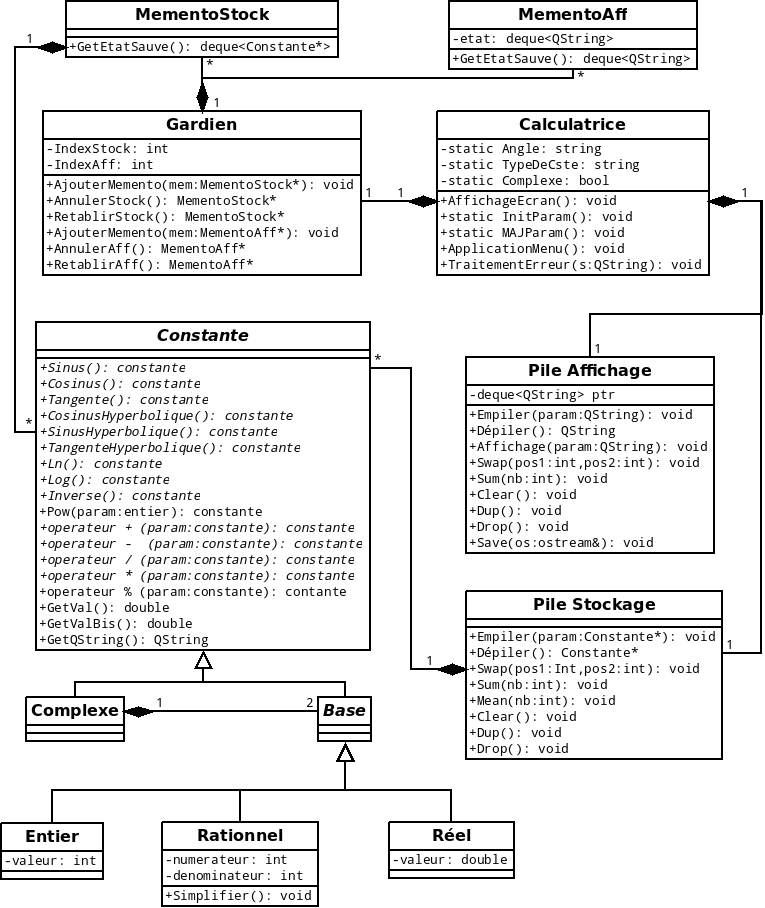
\includegraphics[width=16cm]{UMLProjetLO21v3.png}
				\caption{Diagramme de classe de la Calculatrice}
			\end{figure}

	\section{Diagrammes de séquences}
		\begin{figure}[H]
			\center
			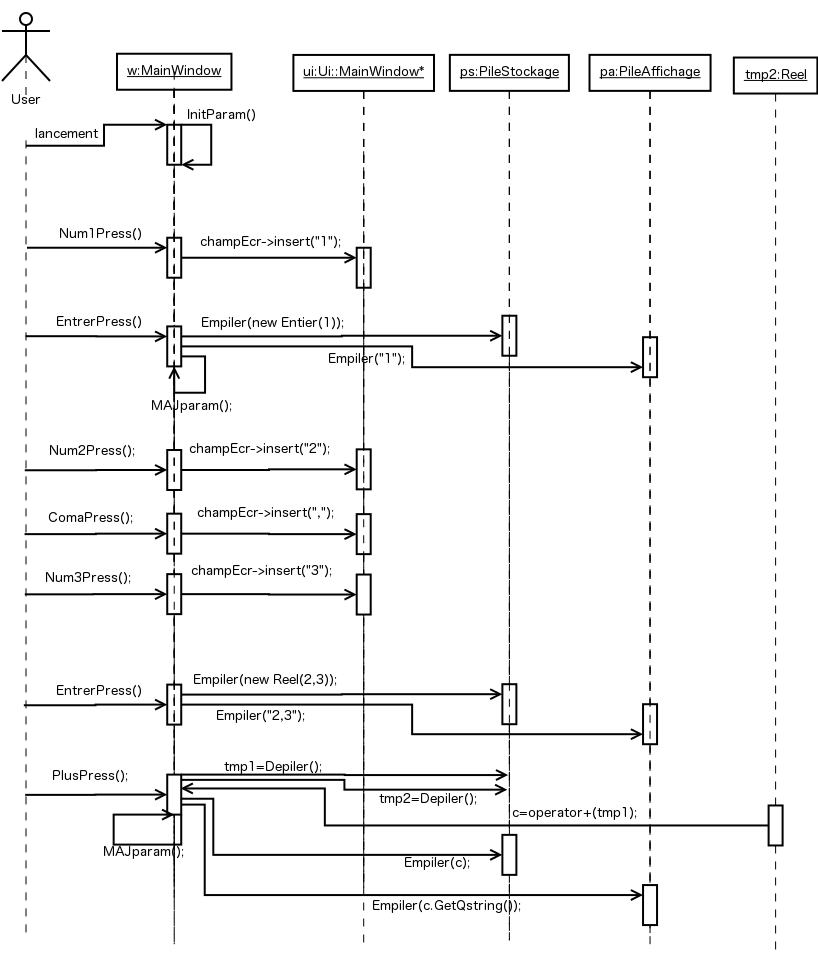
\includegraphics[width=16cm]{diag_seq_1.png}
			\caption{Diagramme de séquence 1}
			\label{Diagramme sequence 1}
		\end{figure}
		
		\paragraph{}Ce diagramme de séquence décrit le lancement de la fenêtre, la saisie de "1", "2,3" , l'appui sur le bouton "+" par l'utilisateur, puis l'addition des deux valeurs.

		\begin{figure}[H]
			\center
			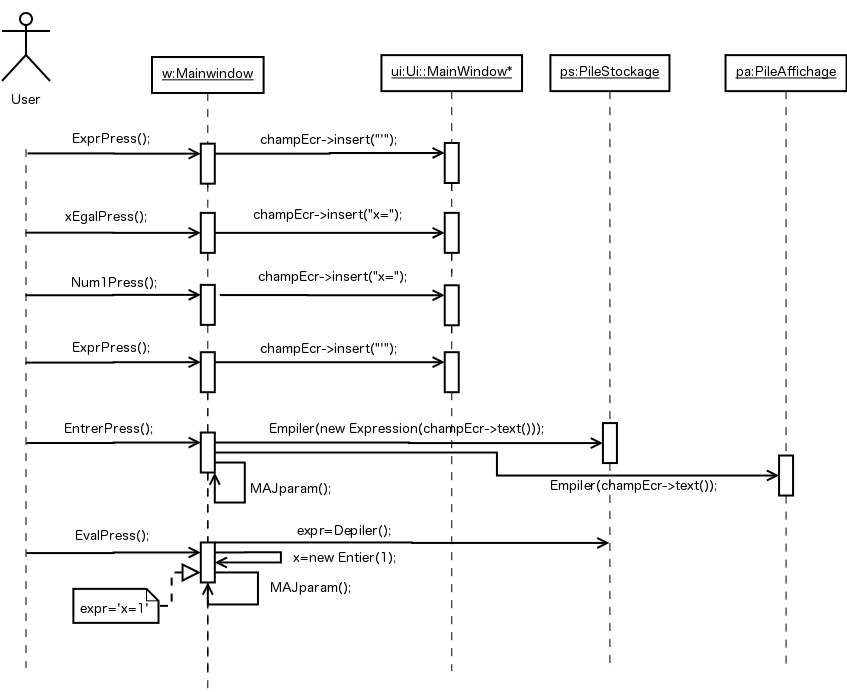
\includegraphics[width=16cm]{diag_seq_2.png}
			\caption{Diagramme de séquence 2}
			\label{Diagramme sequence 2}
		\end{figure}
		
		\paragraph{}Ce diagramme de séquence décrit le lancement de la fenêtre, la saisie de 'x=1', puis l'évaluation de l'expression et la sauvegarde de la valeur 1 dans la variable x.

\chapter{Implémentation}

	\section{Paramètres utilisateur}
		\paragraph{}L'utilisateur dispose d'un menu "Paramètres" lui permettant :
		\begin{itemize}
			\item{De changer le type de constante}
			\item{D'activer ou désactiver le clavier}
			\item{D'activer ou désactiver le mode complexe}
			\item{De choisir l'unité d'angle pour les fonctions cos, sin, tan, cosh, sinh et tanh}
		\end{itemize}
		
		\paragraph{}Le type de constante à été implementé pour une évolution future possible. Ainsi nous avons choisi de garder le type le plus riche en résultat d'une opération et donc de ne pas tenir compte de ce menu. % LOL

	\section{Variable utilisateur}
		\paragraph{}L'initialisation de la variable utilisateur x se fait par l'intermédiaire d'une expression de la forme 'x=valeur'. Après évaluation (bouton "Eval"), cette expression initialise la variable x avec la valeur spécifiée, qui peut-être de type Entier, Rationnel, Réel ou Complexe. Ce comportement est décrit dans la figure \ref{Diagramme sequence 2}.

		\paragraph{}La variable x sera ensuite accessible en tapant directement x ou par l'intermédiaire du bouton "x".

	\section{Sauvegarde et restauration de contexte}
		\paragraph{}A l'ouverture du programme, une méthode est lancée permettant la restauration du contexte de la Calculatrice : il s'agit des piles, des valeurs des menu et de la valeur de la variable utilisateur si elle a été initialisée. Cette méthode interroge un fichier "param.txt" contenant les données du contexte. Si il s'agit de la première ouverture du programme, le fichier est initialisé avec des valeurs par défaut.

		\paragraph{}A chaque entrée de l'utilisateur ou modification des paramètres, une méthode est lancée pour mettre à jour le ficher.

	\section{Historique}
		\paragraph{}Notre historique est implémenté avec le design pattern memento. Ainsi il est composé de trois classes, le Memento qui est une version de sauvegarde, le gardien qui est composé de plusieurs mementos et la pile est l'élément à sauvegarder. 
		
		 \paragraph{}Lors d’un changement de la pile, un memento est crée pour chacune des deux piles. Ce memento est une copie de la pile, Il est ensuite empilé dans le gardien. Les fonctions annuler et rétablir naviguent dans les mementos du gardien pour récupérer ces mémentos et utilise une méthode des pile pour lire et récupérer l'information contenu dans le memento.
		 
	\section{Exceptions}
		\paragraph{}Nous avons choisi d'implémenter qu'une seule classe Exception. Cette classe est composé d'une chaine de caratères et d'une méthode renvoyant celle-ci. Lors de l'execution d'un \emph{throw} une instance d'erreur est créée et la chaine de caractère est envoyé par la méthode de la classe Exception. Cette chaine de caractère est ensuite prise en charge par une méthode de la calculatrice pour l'affichage dans le champ texte prévu à cet effet.
		
	\section{Méthodes de Constante et ses classes filles}
		\paragraph{}Pour les opérateurs utilisables avec plusieurs types de données, par exemple l'opérateur + peut-être utilisés avec les types Entier, Réel, Rationnel, Complexe et Expression, nous avons d'abord défini une méthode de Constante permettant d'appeler la bonne méthode de ses classes filles.

		\paragraph{}Toutes les méthodes ont ensuite dues être implémentées pour tous les types de données. Nous avons fait le choix de toujours renvoyer le type le plus riche. Par exemple, l'addition d'un entier et d'un réel renverra toujours un réel, de même la soustraction d'un rationnel et d'un complexe renverra un complexe.\footnote{Pour les opérations entre les types Rationnel et Réel, nous avons choisi de toujours renvoyer un Réel, méme si il ne s'agit pas du type le plus riche, du fait que nous ne pouvons pas convertir un Réel en Rationnel sans perdre d'information sur celui-ci.} Les méthodes qui n'acceptait pas le type de données, par exemple l'opérateur mod (modulo) n'accepte que les entiers, renvoient des exceptions.

	\section{Piles}
		\paragraph{}Nous avons fait le choix d'utiliser deux piles. Leur contenu est identique à la différence que la pile de stockage contient des Constantes alors que la pile d’affichage contient cette la valeur de cette constante sous forme de QString.
		
		\paragraph{}La pile d’affichage permet un affichage sur l’écran simplifié, ainsi il n'est pas nécessaire de parcourir la pile de stockage en entier et de transformer à chaque itération les constantes en QString. De plus, cette pile d'affichage sert à sauvegarder le contexte de manière plus aisée, en effet il est plus facile d'écrire un QString dans un fichier qu'une Constante.
		
		\paragraph{}Enfin, nous avons utilisé la STL pour créer nos piles. La structure deque a été utilisée, ainsi nous avons adapter cette structure à travers la pile pour une utilisation spécifique à nos problématiques.
		
	\section{Opérateur binaires}
			\paragraph{}Pour la majorité de nos opérateurs binaires, nous avons fait le choix d'utiliser le design pattern Template Method. Ainsi nous traitons chaque opération binaire par la classe Constante qui délègue le calcule dans les surcharges des classes filles. Cela évite d’utiliser des \emph{dynamic\_cast} de manière excessive et permet de factoriser le code.

	\section{Types de données}
		\paragraph{}Nous avons représenté nos types en nous inspirant du design pattern Composite, ainsi nous avons une classe abstraite Constante dont hérite tout les types de données. De plus les méthodes sont virtuelles pures et donc quelque soit la classe fille de Constante les méthodes sont identiques et s'appellent de la même façon.
		
	\section{Utilisation des Singletons}
		\paragraph{}Pour permettre de respecter la constrainte d'unicité de que nous avons décrit dans l'UML, nous avons choisi d'implementer les classes Gardien, Pile de Stockage et Pile d'Affichage avec le design pattern singleton.
		
\chapter{Améliorations et difficultés}

	\section{Critiques de conception}
		\paragraph{}Bien que la Pile d'Affichage possède des aspect pratique évoqué précédemment, elle contient également des contraintes. Ces dernières résident surtout dans l'obligation de créer un memento dédié et de faire fonctionner la classe Gardien de manière parallèle afin d'assurer la cohérence des données présentes dans les deux piles.
		
		\paragraph{}De plus nous n'avons pas utilisé le design pattern MVC, ainsi les contrôles et les affichages sont à la fois diséminées dans la structure et dans le cas de la Classe calculatrice ils sont fusionnés, ce qui engendre un problème de clarification stricte des rôles et des actions réalisées.

		\paragraph{}Enfin, nous n'avons pas réussi à éviter une surcharge massive des opérateurs binaires en prenant en compte chaque situations de calcul, cela a pour effet d'encombrer le code et engendre un manque d'efficacité dans l'implémentation.
		
	\section{Difficultés rencontrées}
		\paragraph{}Nous avons vite pris en main Git pour éviter les problèmes de versions qui se sont posés dans les deux premières semaines.
		
		\paragraph{}Le projet aurait demander plus de temps pour une implémentation correcte. En effet, peu de design pattern ont été abordé en cours se qui demandait un gros effort de recherche personnel pour réaliser une projet implémenté de façon propre.
		
\chapter*{Conclusion}
	\paragraph{}Ce projet nous aura permis de prendre conscience des difficultés et des problématiques lors de la conception et l'implémentation logiciel\footnote{Qui est bien plus vaste que LO21} et a commencer à nous familiariser avec celles-ci. Nous avons de plus découvert de nombreuses méthodes de programmation à travers les design pattern, enfin l'apprentissage d'un logiciel de gestion de versions à été très utile pour le travail collaboratif.

%\listoffigures

\end{document}
